\section{MRI Data Acquisition}
\label{sec:mri_acquisition}

MRI sessions followed a multimodal acquisition framework that was broadly consistent
across complete visits, although the exact set, number, and order of acquisitions varied
according to the study protocol and participant group. Complete examination sessions
typically lasted approximately 115--135\,min. The description below summarizes the overall
organization of the examination, while detailed acquisition parameters are provided
separately in Table~\ref{tab:mri_acq_parameters}.

%% MRI acquisition parameters (representative values from released BIDS sidecars).
%% Companion to the session-organisation paragraph in sec:mri_acquisition.
%% Diffusion rows align with docs/diffusion/diffusion_acquisition_parameters.tsv.
\begin{table}[htbp]
\centering
\caption{MRI acquisition parameters for the principal sequences in the release.
Values are representative parameters taken from packaged BIDS JSON sidecars
(Siemens Prisma~3\,T, 64-channel head/neck coil). Exact run counts and console
order varied across sessions; \texttt{run} indices are assigned at conversion.
Diffusion rows distinguish raw gSlider slab geometry from the reconstructed
1\,mm \texttt{Normalize\_DWI} derivative. Localizer series were acquired for
prescription but are not packaged in the release.}
\label{tab:mri_acq_parameters}
\footnotesize
\setlength{\tabcolsep}{3.5pt}
\renewcommand{\arraystretch}{1.15}
\begin{adjustbox}{max width=\textwidth,center}
\begin{tabular}{@{}>{\raggedright\arraybackslash}p{2.6cm}
                >{\raggedright\arraybackslash}p{2.4cm}
                >{\raggedright\arraybackslash}p{2.1cm}
                c
                >{\raggedright\arraybackslash}p{2.0cm}
                >{\raggedright\arraybackslash}p{3.6cm}@{}}
\toprule
\textcolor{headergray}{\textbf{Sequence}} &
\textcolor{headergray}{\textbf{ProtocolName}} &
\textcolor{headergray}{\textbf{Voxel size (mm)}} &
\textcolor{headergray}{\textbf{TR / TE (/ TI)}} &
\textcolor{headergray}{\textbf{FA / accel.}} &
\textcolor{headergray}{\textbf{Notes}} \\
\midrule
\multicolumn{6}{@{}l}{\textit{Anatomical}} \\
\midrule
T1w MPRAGE & \texttt{T1w\_MPR} & $0.8$ iso & $2500$ / $2.22$ / $1000$\,ms & $8^\circ$; iPAT\,2 & Typically two runs/session; \texttt{run-02} usually reconstructed with Siemens \texttt{NORM} \\
\rowcolor{tablealt}
WMn MPRAGE & \texttt{WMn\_MPRAGE\_sagittal} & $1.0$ iso & $4000$ / $3.82$ / $500$\,ms & $7^\circ$; iPAT\,2 & White-matter-nulled; usually \texttt{run-03\_T1w} \\
3D FLAIR & \texttt{Sag Flair 3D-0.8} & $0.8$ iso & $6000$ / $357$ / $2200$\,ms & $120^\circ$; iPAT\,2 & One run/session in most visits \\
\rowcolor{tablealt}
B1 map & \texttt{tfl\_b1map\_1mmiso} & $\sim 3.4\times3.4\times10$ & $4000$ / $1.83$\,ms & $8^\circ$ & 15 slices (thickness 8\,mm, spacing 10\,mm); gSlider B1 calibration (\texttt{TB1TFL}) \\
\midrule
\multicolumn{6}{@{}l}{\textit{Functional BOLD (MB8 EPI; tasks share geometry)}} \\
\midrule
BOLD (all tasks) & \texttt{REST*}/\texttt{Movie*}/\texttt{fMRI*}/\texttt{Control*} & $2.0$ iso & $937$ / $37$\,ms & $52^\circ$; MB\,8 & Matrix $104\times104\times88$; BW $\sim$2290\,Hz/Px; PE mainly AP (some control runs PA). Representative lengths: rest $\sim$320, movie $\sim$210, fmri $\sim$226, control $\sim$20 vols \\
\midrule
\multicolumn{6}{@{}l}{\textit{Field maps}} \\
\midrule
Spin-echo EPI fmap & \texttt{SpinEchoFieldMap\_AP/PA} & $2.0$ iso & $9710$ / $66$\,ms & $90^\circ$ & Opposing PE (\texttt{dir-AP}/\texttt{dir-PA}); matched to BOLD FOV/matrix for distortion correction \\
\midrule
\multicolumn{6}{@{}l}{\textit{Diffusion}} \\
\midrule
gSlider-SMS AP & \texttt{gsld\_76dir\_b2000\_1mmiso\_AP} & Raw $1\times1\times5$ (30 slabs); recon.\ $1$ iso & $3500$ / $75$\,ms & $90^\circ$; MB\,2; iPAT\,3; PF\,6/8 & Multi-shell $b=0/1000/2000$\,s/mm$^2$. Raw series retain RF encodings (modal 385 time points). Analysis-ready: $4\,b0+37+36=77$ vols in \texttt{Normalize\_DWI} \\
\rowcolor{tablealt}
gSlider PA $b=0$ & \texttt{gsld\_75TE\_PA\_3b0} & Raw $1\times1\times5$ & $3500$ / $75$\,ms & $90^\circ$; MB\,2; iPAT\,3; PF\,6/8 & Reverse-PE $b=0$ references (modal 5 vols); for topup \\
RESOLVE trace AP & \texttt{resolve\_\ldots{}1.4iso\_AP} & $\sim 1.38\times1.38\times1.82$ & $4140$ / $51$\,ms & $180^\circ$; iPAT\,3 & Clinical RESOLVE; $b=0/1000$\,s/mm$^2$ (modal 15 vols); TRACEW products also released \\
\rowcolor{tablealt}
RESOLVE PA & \texttt{resolve\_\ldots{}1.4iso\_PA} & $\sim 1.38\times1.38\times1.82$ & $\sim 24.8$\,s / $51$\,ms & $180^\circ$; iPAT\,3 & Primarily reverse-PE $b=0$ (modal 3 vols) \\
\bottomrule
\end{tabular}
\end{adjustbox}
\end{table}


\subsection{MRI Scanner}

% Write here.


\subsection{Anatomical MRI}

% Write here. Cite Table~\ref{tab:mri_acquisition} for laboratory series$\rightarrow$BIDS filename mapping.

%% MRI acquisition protocol: laboratory SeriesDescription → BIDS
%% Layout matches reports/pi_pipeline_briefing/figures/Table_MRI_acquisition_protocol_lab_to_bids.png
\begin{table}[htbp]
\centering
\caption{MRI acquisition protocol: laboratory SeriesDescription mapped to BIDS datatype and general filename pattern (single session, console order). Run index $<$N$>$ is assigned at conversion and may differ from acquisition order. Full form: \texttt{sub-<ID>\_ses-<01|02>\_<entities>\_<suffix>.nii.gz}.}
\label{tab:mri_acquisition}
\footnotesize
\setlength{\tabcolsep}{4pt}
\renewcommand{\arraystretch}{1.22}
%% Shrink only if the 11pt/wide-figure layout exceeds manuscript \textwidth.
\begin{adjustbox}{max width=\textwidth,center}
\begin{tabular}{@{}c l c l@{}}
\toprule
\textcolor{headergray}{\textbf{\#}} &
\textcolor{headergray}{\textbf{Lab series name}} &
\textcolor{headergray}{\textbf{BIDS datatype}} &
\textcolor{headergray}{\textbf{General BIDS name}} \\
\midrule
1 & \texttt{Localizer} & \texttt{anat} & \texttt{run-\textless{}N\textgreater{}\_localizer} \\
\rowcolor{tablealt}
2 & \texttt{fMRI1\_AP} & \texttt{func} & \texttt{task-fmri\_run-\textless{}N\textgreater{}\_bold} \\
3 & \texttt{fMRI2\_AP} & \texttt{func} & \texttt{task-fmri\_run-\textless{}N\textgreater{}\_bold} \\
\rowcolor{tablealt}
4 & \texttt{Control1\_PA} & \texttt{func} & \texttt{task-control\_run-\textless{}N\textgreater{}\_bold} \\
5 & \texttt{fMRI3\_AP} & \texttt{func} & \texttt{task-fmri\_run-\textless{}N\textgreater{}\_bold} \\
\rowcolor{tablealt}
6 & \texttt{fMRI4\_AP} & \texttt{func} & \texttt{task-fmri\_run-\textless{}N\textgreater{}\_bold} \\
7 & \texttt{Movie1\_AP} & \texttt{func} & \texttt{task-movie\_run-\textless{}N\textgreater{}\_bold} \\
\rowcolor{tablealt}
8 & \texttt{Movie2\_AP} & \texttt{func} & \texttt{task-movie\_run-\textless{}N\textgreater{}\_bold} \\
9 & \texttt{SpinEchoFieldMap\_AP} & \texttt{fmap} & \texttt{dir-AP\_run-\textless{}N\textgreater{}\_epi} \\
\rowcolor{tablealt}
10 & \texttt{SpinEchoFieldMap\_PA} & \texttt{fmap} & \texttt{dir-PA\_run-\textless{}N\textgreater{}\_epi} \\
11 & \texttt{Movie3\_AP} & \texttt{func} & \texttt{task-movie\_run-\textless{}N\textgreater{}\_bold} \\
\rowcolor{tablealt}
12 & \texttt{Movie4\_AP} & \texttt{func} & \texttt{task-movie\_run-\textless{}N\textgreater{}\_bold} \\
13 & \texttt{REST1\_AP} & \texttt{func} & \texttt{task-rest\_run-\textless{}N\textgreater{}\_bold} \\
\midrule
\textbf{*} & & & \\
\midrule
\rowcolor{tablealt}
14 & \texttt{Localizer} & \texttt{anat} & \texttt{run-\textless{}N\textgreater{}\_localizer} \\
15 & \texttt{T1w\_MPR} & \texttt{anat} & \texttt{run-\textless{}N\textgreater{}\_T1w} \\
\rowcolor{tablealt}
16 & \texttt{Control2\_AP} & \texttt{func} & \texttt{task-control\_run-\textless{}N\textgreater{}\_bold} \\
17 & \texttt{Control3\_PA} & \texttt{func} & \texttt{task-control\_run-\textless{}N\textgreater{}\_bold} \\
\rowcolor{tablealt}
18 & \texttt{SpinEchoFieldMap\_AP} & \texttt{fmap} & \texttt{dir-AP\_run-\textless{}N\textgreater{}\_epi} \\
19 & \texttt{SpinEchoFieldMap\_PA} & \texttt{fmap} & \texttt{dir-PA\_run-\textless{}N\textgreater{}\_epi} \\
\rowcolor{tablealt}
20 & \texttt{gsld\_76dir\_b2000\_1mmiso\_AP} & \texttt{dwi} & \texttt{run-\textless{}N\textgreater{}\_dwi} \\
21 & \texttt{gsld\_75TE\_PA\_3b0} & \texttt{dwi} & \texttt{run-\textless{}N\textgreater{}\_dwi} \\
\rowcolor{tablealt}
22 & \texttt{tfl\_b1map\_1mmiso} & \texttt{anat} & \texttt{run-\textless{}N\textgreater{}\_TB1TFL} \\
23 & \texttt{resolve\_3scan\_trace\_tra\_p3\_160\_1.4iso\_AP} & \texttt{dwi} & \texttt{run-\textless{}N\textgreater{}\_dwi} \\
\rowcolor{tablealt}
24 & \texttt{resolve\_3scan\_trace\_tra\_p3\_160\_1.4iso\_PA} & \texttt{dwi} & \texttt{run-\textless{}N\textgreater{}\_dwi} \\
25 & \texttt{Sag Flair 3D-0.8} & \texttt{anat} & \texttt{run-\textless{}N\textgreater{}\_FLAIR} \\
\rowcolor{tablealt}
26 & \texttt{WMn\_MPRAGE\_sagittal} & \texttt{anat} & \texttt{run-\textless{}N\textgreater{}\_T1w} \\
\bottomrule
\end{tabular}
\end{adjustbox}

\vspace{4pt}
\begin{flushleft}
\footnotesize
\textbf{*} Anterior part of the head coil added, after which the localizer is repeated.
\end{flushleft}
\end{table}


\subsection{Functional MRI}

% Write here.


\subsection{Field Maps}

% Write here.


\subsection{Diffusion MRI}

\begin{figure}[htbp]
\centering
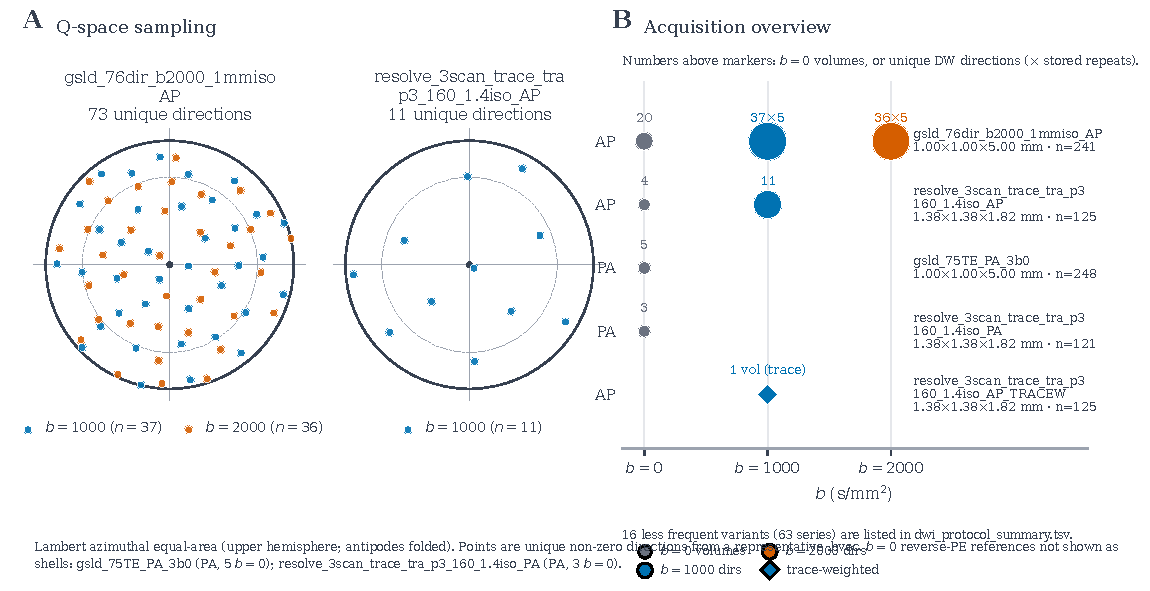
\includegraphics[width=\linewidth]{figures/Figure_DWI_protocols.pdf}
\caption{Diffusion MRI acquisition schemes in the released BIDS dataset. (A)~Angular distribution of unique non-zero diffusion-encoding directions from representative \texttt{.bvec} files, shown as a Lambert azimuthal equal-area projection of the upper hemisphere (antipodal directions folded). \texttt{gsld\_76dir\_b2000\_1mmiso\_AP} [AP: $b=1000$ ($n=37$ unique directions), $b=2000$ ($n=36$ unique directions)]; \texttt{resolve\_3scan\_trace\_tra\_p3\_160\_1.4iso\_AP} [AP: $b=1000$ ($n=11$ unique directions)]. Reverse-phase-encoding $b=0$ series (\texttt{gsld\_75TE\_PA\_3b0} [PA]; \texttt{resolve\_3scan\_trace\_tra\_p3\_160\_1.4iso\_PA} [PA]) are reference images and are not plotted as diffusion shells. (B)~Protocol-level summary of $b$-value shells, unique angular samples per shell, $b=0$ volume counts, voxel size, phase-encoding direction, and number of magnitude series for schemes represented in $\geq$20 series. The figure is derived from 923 released DWI NIfTI files in 131 sessions and shows unique acquisition schemes rather than every individual series. Where a gradient table stores repeated encodings of the same direction, panel~A plots unique directions and panel~B reports the observed repeat factor. 16 less frequent variants (truncated shells, alternate voxel size, missing phase-encoding metadata, or shim/PE differences) are tabulated in \texttt{dwi\_protocol\_summary.tsv}.}
\label{fig:dwi_protocols}
\end{figure}


% Write here. Cite Fig.~\ref{fig:dwi_protocols}.


\subsection{Physiological Recordings}

% Write here.

